\documentclass[a4paper,twoside, 11pt, leqno]{scrartcl}

\input{../head.tex}
\title{Pensar jugando}
\author{}
%\date{}

\usepackage{pifont,skak}

\makeatletter\let\Title\@title\makeatother
\makeatletter\let\Author\@author\makeatother



\usepackage{tikz}
\usetikzlibrary{%
  lindenmayersystems,
  decorations.pathmorphing,
  decorations.markings,
  shapes.geometric,
  calc%
}
\tikzset{
  tinsel/.style={
    #1,
    rounded corners=10mm,
    ultra thin,
    decorate,
    decoration={
      snake,
      amplitude=.1mm,
      segment length=10,
    }
  },
  baubles/.style={
    decorate,
    decoration={
      markings,
      mark=between positions .3 and 1 step 2cm
      with
      {
        \pgfmathsetmacro{\brad}{2 + .5 * rand}
        \path[shading=ball,ball color=#1] (0,0) circle[radius=\brad mm];
      }
    }
  },
  lights/.style={
    decorate,
    decoration={
      markings,
      mark=between positions 0 and 1 step 1cm
      with
      {
        \pgfmathparse{rand > 0 ? "dart" : "kite"}
        \let\lshape\pgfmathresult
         \pgfmathsetmacro{\tint}{100*rnd}
        \node[rotate=90,\lshape,shading=ball,inner sep=1pt,ball color=red!\tint!yellow] {};
      }
    }
  }
}


\newcommand{\vol}{Vol. I, No. 6}
%\renewcommand{\seccol}{scicol!60}
\renewcommand{\seccol}{cscc}

\newcounter{row}
\newcounter{col}

\newcommand\setrow[9]{
  \setcounter{col}{1}
  \foreach \n in {#1, #2, #3, #4, #5, #6, #7, #8, #9} {
    \edef\x{\value{col} - 0.5}
    \edef\y{9.5 - \value{row}}
    \node[anchor=center] at (\x, \y) {\n};
    \stepcounter{col}
  }
  \stepcounter{row}
}


\begin{document}

\setcounter{page}{26}
\thispagestyle{scrplain}


\begin{multicols}{2}

  \cappar En este número os damos la solución al desafío del anterior número y os dejamos un nuevo desafío basado en un programa de televisión americano y una nueva partida. Al final os dejamos un recortable para que compartan con los mas pequeños. ¡Disfrútenlo!


\section*{Desafíos fín de año}
\subsection{Desafío Día de la Familia}
The tourist has come to the Moscow by train.  All-day-long he wandered
randomly through the streets.  Than he had a supper in the cafe on the
square and decided to return to the station only through the streets
that he has passed an odd number of times.
Prove that he is always able to do that.
\subsection{Desafío año nuevo}
\begin{enumerate}
\item Una cierta comité se ha reunido 40 veces. Hubo 10 miembros en
todas las reuniones. Ni una sola pareja se ha reunido en las reuniones dos veces.
Demuestre que había no menos de 60 miembros en el comité.
\item Demuestra que no se puede construir más de 30 subcomités de 5 miembros de la comisión de 25 miembros, sin par de subcomités que tienen más de un miembro común.
\end{enumerate}
{\bf Las soluciones en el próximo número.}
\section*{\textcolor{redsol}{Soluciones del número anterior}}
\subsection{El desafío: Monty Hall extendido}
Esta vez, vamos a daros la solución al problema de Monty Hall con \textbf{cuatro} puertas, una de las cuales esconde un premio que quieres ganar y cuando eliges por primera vez, el presentador te abre dos puertas malas y te da a elegir entre tu puerta y la que queda sin abrir.

 Cuando eliges una puerta, tienes $1/4$ de probabilidad de acertar, y por lo tanto, tienes $3/4$ de probabilidades de haber fallado (evidentemente, esta probabilidad se reparte entre las tres puertas que no se han elegido, cada una con $1/4$).

Cuando el presentador abre las dos puertas malas, tu probabilidad de haber acertado no cambia en absoluto, sigue siendo $1/4$. Por lo tanto, tampoco cambia la probabilidad de que hayas fallado, que sigue siendo $3/4$. Por lo tanto, tenemos dos puertas. El premio está en la tuya con probabilidad $1/4$ y debe estar en la otra con probabilidad $3/4$, de modo que lo más recomendable sería cambiar de puerta.
%\end{multicols}

\begin{center}
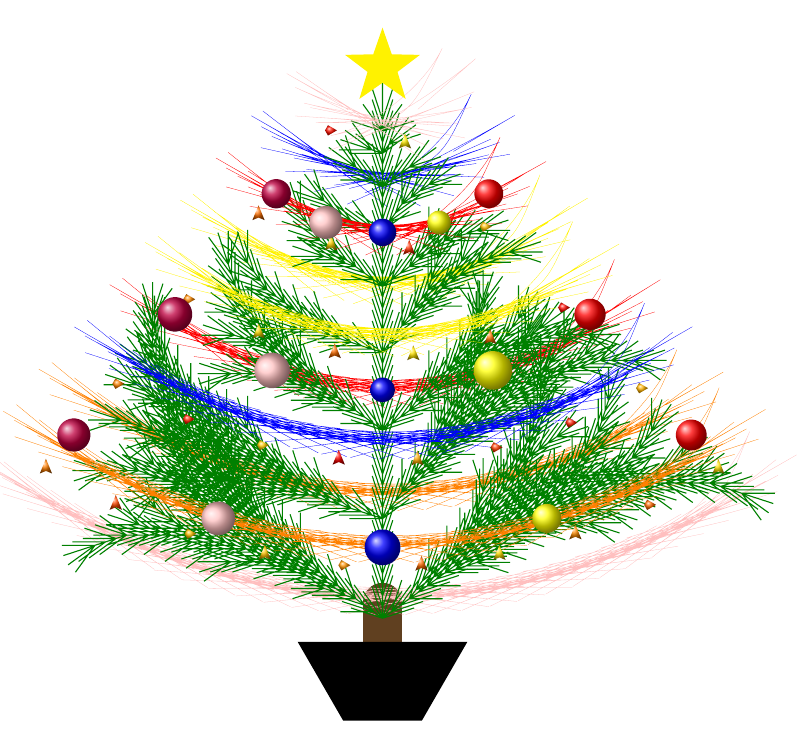
\begin{tikzpicture}
\coordinate (star) at (0,-1);
\path (star) +(-50:7) coordinate (rhs) +(-130:7) coordinate (lhs);
\draw[brown!50!black,line width=5mm,line cap=round] (star) ++(-90:6.8) -- ++(0,-1) coordinate (base);
\node[scale=-1,trapezium,fill=black,minimum size=1cm] at (base) {};
\foreach \height/\colour in {%
  .2/blue,
  .4/yellow,
  .6/red,
  .8/orange,
  1/pink%
} {
  \draw[tinsel=\colour] ($(star)!\height!(lhs)$) to[bend right] ($(star)!\height!(rhs)$);
}
\path (star);
\pgfgetlastxy{\starx}{\stary}
\begin{scope}[xshift=\starx,yshift=\stary,yshift=-7cm]
\draw[color=green!50!black, l-system={rule set={S -> [+++G][---G]TS,  G -> +H[-G]L, H -> -G[+H]L, T -> TL, L -> [-FFF][+FFF]F}, step=4pt, angle=18, axiom=+++++SLFFF, order=11}] lindenmayer system -- cycle;
\end{scope}
\foreach \height/\colour in {%
  .1/pink,
  .3/red,
  .5/yellow,
  .7/blue,
  .9/orange%
} {
  \draw[tinsel=\colour] ($(star)!\height!(lhs)$) to[bend right] ($(star)!\height!(rhs)$);
}
\foreach \height in {.15,.35,...,1} {
  \draw[lights]  ($(star)!\height!(lhs)$) to[bend right] ($(star)!\height!(rhs)$);
}
\foreach \angle/\colour in {
  -50/red,
  -70/yellow,
  -90/blue,
  -110/pink,
  -130/purple%
} {
  \draw[baubles=\colour] (star) -- ++(\angle:7);
}
\node[star,star point ratio=2.5,fill=yellow,minimum size=1cm] at (star) {};
\end{tikzpicture}
\LARGE{\textcolor{red}{Feliz Natal}}
\end{center}


\end{multicols}
\newpage


%%% Local Variables:
%%% mode: latex
%%% TeX-master: "jugando"
%%% End:





%\bibliographystyle{plain}
%\bibliography{catenaria}
\end{document}
%%% Local Variables: 
%%% mode: latex
%%% TeX-master: t
%%% End: 
